\documentclass{article} % For LaTeX2e
\usepackage{iclr2026_conference,times}

% Optional math commands from https://github.com/goodfeli/dlbook_notation.
\input{math_commands.tex}

\usepackage[utf8]{inputenc}
\usepackage[T1]{fontenc}
\usepackage{amsmath, amssymb, amsfonts, amsthm, mathtools}
\usepackage{algorithm}
\usepackage{algpseudocode}
\usepackage{enumitem}
\usepackage[most]{tcolorbox}
\usepackage{url}
\usepackage{booktabs}
\usepackage{nicefrac}
\usepackage{microtype}
\usepackage{xcolor}
\setcitestyle{numbers,square}
\usepackage{hyperref}
\usepackage{bm}
\usepackage{pgfplots}
\pgfplotsset{compat=1.18}
\usepackage{subcaption}

\theoremstyle{plain}
\newtheorem{theorem}{Theorem}[section]
\newtheorem{lemma}[theorem]{Lemma}
\newtheorem{proposition}[theorem]{Proposition}
\newtheorem{corollary}[theorem]{Corollary}
\theoremstyle{definition}
\newtheorem{assumption}{Assumption}[section]
\newtheorem{definition}{Definition}[section]

\title{Planning Emerges from Reinforcement \\ Learning with Relational Latent States}

\author{{Armin Sommer} \\
{ETH Zurich, Switzerland}\\
{\texttt{sommera@ethz.ch}}}

\newcommand{\fix}{\marginpar{FIX}}
\newcommand{\new}{\marginpar{NEW}}

%\iclrfinalcopy % Uncomment for camera-ready version, but NOT for submission.
\newenvironment{ack}{\section*{Acknowledgments}}{}

\begin{document}

\maketitle

\begin{abstract}
It has been observed empirically that planning mechanisms can emerge from
model-free reinforcement learning. While the planning algorithms of specific
cases have been analyzed, the question of when, or due to which inductive
bias, planning will emerge has been left unanswered. In this work, we show
that when a neural agent has latent states that learn relations between them,
such as convolutional hidden states or attention blocks, the agent can learn
to tie these states to environment states and then plan over the learned state
graph: a learned \emph{policy-evaluation operator} computes a value field --- a
latent from which the value is decodable --- and the recurrence refines the
\emph{decision} read from it; with the critic's value learning, this realizes
generalized policy iteration in latent space.
\end{abstract}

\section{Introduction}
\label{sec:intro}

A striking empirical observation is that agents trained purely by model-free
reinforcement learning can nonetheless behave as if they \emph{plan}. Recurrent
convolutional agents on Sokoban solve more levels when given extra
``thinking'' steps before acting, pause to deliberate at the start of hard
levels, and generalize to larger out-of-distribution puzzles
\citep{guez2019investigation}; their internal activations have been decoded
into explicit look-ahead --- which box will be pushed in which direction, where
the agent will go --- that forms over internal computation and causally
determines the action taken \citep{bush2025interpreting,taufeeque2024planning}.
None of these agents were given a model, a search procedure, or a planning
objective.

What this line of work establishes is \emph{which} algorithm particular
trained agents run. What it leaves open is \emph{when} planning emerges:
which inductive bias of the architecture is responsible, and whether the same
mechanism should be expected beyond the specific convolutional networks
studied. That is the question this paper answers.

Our answer is that the responsible inductive bias is \emph{relational latent
states}: a backbone whose substrate is a pool of weight-tied latent cells
exchanging messages along learned relations, of which convolutional hidden
grids and attention blocks are the two common instances. Trained by
actor--critic RL with a cell budget matching the state space, such a substrate
acquires two properties, neither of which is hand-built:
\begin{enumerate}[leftmargin=1.5em,itemsep=2pt,topsep=2pt]
\item \textbf{Binding.} Distinct latent cells come to represent distinct
environment states --- the network learns an (approximately) injective map from
states to cells whose content depends only on the local configuration of that
state.
\item \textbf{Transition-respecting routing.} The content-based routing comes
to connect a cell to exactly the cells of the states reachable from it by one
transition, so the effective graph over cells coincides with the environment's
transition graph $\mathcal N$: a \emph{learned state graph}.
\end{enumerate}

Once these hold, planning follows from the architecture's own recurrence. Our
central theoretical result (Section~\ref{sec:planning}) is that in a bound,
localized configuration the thinking loop is not a black box: it applies a learned
\emph{policy-evaluation operator} along the graph to a value-decodable decision
statistic, and a localized head reads a policy from it. The operator's fixed point
is a value field; the network may reach it by iterating across ticks or compile it
into a single step (empirically the latter), and what more thinking then refines is
the \emph{decision} at the head, settling it toward greedy --- most for the hardest
states. Refinement of the decision within a thinking sweep and value
learning by temporal differences across environment steps together constitute
\emph{generalized policy iteration} on the learned state graph. We stress that one
need not attribute the latent loop to a particular half of policy iteration:
whether it is best read as policy evaluation (propagating the current value) or as
policy improvement (a look-ahead backup) depends only on how selective the learned
routing is, and the two are endpoints of one spectrum. The architecture-level
claim is invariant to that choice --- a generic relational recurrence, supplied
only with RL signal, comes to run this refinement-and-readout loop over a graph it
has itself learned.

The answer also delimits what must, and need not, be built in. A convolutional
core hard-masks its routing to a local stencil, so the state graph is supplied
by the architecture; a core with dense, content-based routing must
\emph{learn} which cells are neighbours, and we find that it does, routing
precisely to the transition-feasible cells. Planning emerges in both. The
operative ingredient is therefore the relational latent-state substrate
itself; a locality mask is an inductive convenience that accelerates the
symmetry-breaking, not a precondition for it.

\textbf{Contributions.} (i) We identify relational latent states as the
inductive bias behind emergent planning, and formalize the configuration that
training drives them to: a \emph{binding} of latent cells to environment
states with localized decision statistics (Section~\ref{sec:binding}).
(ii) We show that, in this configuration, the thinking loop realizes a
policy-evaluation operator over the learned graph (Section~\ref{sec:planning},
Proposition~\ref{prop:improvement}) whose value field the trained network largely
\emph{amortizes}, and additional thinking refines the \emph{decision} read from it
--- generalized policy iteration in latent space, without committing the loop to a
specific half or to iterating vs.\ amortizing the evaluation.
(iii) We verify by mechanistic interpretation that a relational core whose
routing is fully learned (instantiated by attention) acquires both the binding
and a routing that recovers $\mathcal N$ --- in the masked and the dense case
alike --- exhibiting the propagating plan field that prior work decodes from
convolutional planners (Section~\ref{sec:empirics}).



\section{Preliminaries}
\label{sec:prelim}

\textbf{Goal-conditioned setting.} Consider a deterministic Markov Decision
Process $(\mathcal S,\mathcal A,\mathcal T,\mathcal R)$, with $\mathcal S$ a
finite state set, $\mathcal A$ a finite action set,
$\mathcal T:\mathcal S\times\mathcal A\to\mathcal S$ a deterministic transition
map, and $\mathcal R:\mathcal S\to\mathbb R$ a reward. The task fixes a goal
state $s_{\text{goal}}\in\mathcal S$; reward is sparse and terminal, collected
on entering $s_{\text{goal}}$ and zero otherwise.

\textbf{Actor--critic reinforcement learning.} The objective is a policy
maximizing the discounted return
$\mathbb E_\pi\bigl[\sum_{k\geq 0}\gamma^k r_{t+k}\mid s_t=s\bigr]$. A critic
$V^\pi(s)=\mathbb E_\pi\bigl[\sum_{k\geq 0}\gamma^k r_{t+k}\mid s_t=s\bigr]$
estimates this return and is fit by temporal-difference (TD) learning; the
actor is improved against it by the policy gradient
\begin{align}
  \nabla_\phi J(\phi) = \mathbb E_\pi\Bigl[\textstyle\sum_{t}
  \nabla_\phi\log\pi_\phi(a_t\mid s_t)\,\delta_t\Bigr],
\end{align}
where $\delta_t$ is an advantage estimator (e.g. the $n$-step TD error or the
generalized advantage estimate).

\section{Relational Recurrent Core}
\label{sec:core}

We study neural backbones that move information over a relational structure ---
convolutions, graph message passing, or attention. We view such a backbone as a
pool of latent cells exchanging messages, and we deliberately make \emph{no} a
priori correspondence between cells and environment states. We refer to this
substrate --- weight-tied cells whose interactions are given by learned
relations --- as \emph{relational latent states}; it is the inductive bias
whose consequences this paper traces.

\begin{assumption}[Recurrent relational core]
\label{ass:core}
The backbone maintains $N$ latent cells $h_t(i)\in\mathbb R^{n}$. Fix
environment time $t$. Each thinking step $k\in\{0,\dots,K-1\}$ updates every
cell from the cells it is related to,
\begin{equation}
  h_t^{k+1}(i)
  \;=\;
  \bigoplus_{j}
  \alpha^{k}_{ij}\,
  F_{\phi}\bigl(h_t^{k}(j)\bigr),
  \label{eq:update}
\end{equation}
where $F_\phi$ is a learned map producing the message of cell $j$,
$\alpha^{k}_{ij}\geq 0$ is the routing weight of the relation $j\to i$, and
$\oplus$ is an edge-invariant aggregation. The two common instances differ
only in the routing. A \emph{convolution} arranges the cells on a grid, fixes
the support of $\alpha$ to a local stencil, and learns one weight per offset,
$\alpha^{k}_{ij}=c_\phi(j-i)$. \emph{Attention} computes the weights from
content, $\alpha^{k}_{ij}=a_\phi\bigl(h_t^{k}(j),h_t^{k}(i)\bigr)$, over all
pairs. The index $j$ ranges over all cells including $i$ itself, so a cell may
retain its own content through the self-edge. By convention
$h_t^{0}\equiv h_{t-1}^{K}$: the carry between environment steps is the last
thinking state.
\end{assumption}

Two features of \eqref{eq:update} are essential. It is \emph{time-invariant}:
the same parameters act at every thinking step $k$ and environment step $t$,
so the core iterates a single fixed operator. And it is \emph{weight-tied
across cells}: no cell holds private parameters, so any state-dependent
computation must be carried by cell \emph{content} and by the routing
$\alpha$; the core is equivariant over cells (permutation-equivariant when
the routing is content-based, translation-equivariant when it is masked to a
grid stencil). We leave $\oplus$ generic; it is helpful to read it as a
(normalized) weighted sum, with $\max$ and $\operatorname{mean}$ as other
admissible instances. We say the routing is \emph{masked} when its support is
fixed and only the weights on that support are learned, and \emph{dense} when
both the weights and the support --- which cells relate to which --- are
learned: convolution is the masked instance, attention the dense one.


\section{State-Binding and Localized Decision Statistics}
\label{sec:binding}

The architecture fixes no map from cells to states. The environment, for its
part, supplies the structure that such a map could respect. Determinism
induces the \emph{transition graph}
$\mathcal N=\{(s,s')\in\mathcal S\times\mathcal S:\exists\,a\in\mathcal A,\
\mathcal T(s,a)=s'\}$, the directed graph of one-step-reachable states, and it
identifies each action $a$ available at $s$ with the out-neighbour
$s'=\mathcal T(s,a)$ it produces; under this \emph{action--neighbour
identification} a policy $\pi(\cdot\mid s)$ is interchangeably a distribution
over actions and a distribution over the out-neighbours
$\{s':(s,s')\in\mathcal N\}$. We now name the learned configurations in which
the latent cells take on this structure, and around which the rest of the
paper turns.

\begin{definition}[State-indexed configuration / binding]
\label{def:indexed}
A trained core is \emph{state-indexed} on $\mathcal S_0\subseteq\mathcal S$ if
there is an injection $\sigma:\mathcal S_0\to[N]$ such that (i) the content of
cell $\sigma(s)$ is a function of the environment configuration at $s$ alone,
and (ii) routing respects the transition graph: the cell of $s$ receives only
from the cells of its out-neighbours and from itself,
\begin{equation*}
  \alpha_{\sigma(s)\,\sigma(s')}\approx 0
  \quad\text{whenever } (s,s')\notin\mathcal N \text{ and } s'\neq s.
\end{equation*}
The induced \emph{effective graph} over cells then coincides with the
$\sigma$-image of $\mathcal N$, read as ``each state's cell receives from the
cells of its successors.'' We call $\sigma$ the \emph{binding} of latent cells
to environment states.
\end{definition}

\begin{definition}[Localized decision statistics]
\label{def:localized}
The actor and critic are \emph{localized} if there exist shared cellwise
readouts $\rho_\pi,\rho_V$ with
\begin{equation}
  \pi(\cdot\mid s)=\rho_\pi\!\bigl(h_t(\sigma(s))\bigr),
  \qquad
  V^{\pi}(s)=\rho_V\!\bigl(h_t(\sigma(s))\bigr),
  \label{eq:localized}
\end{equation}
for all $s,t$: every decision statistic at $s$ is a function of the single cell
$\sigma(s)$, and, by the action--neighbour identification, $\pi(\cdot\mid s)$
is a distribution over the out-neighbour cells
$\{\sigma(s'):(s,s')\in\mathcal N\}$.
\end{definition}

\textbf{Why binding is the operative condition.} Nothing in
Assumption~\ref{ass:core} ties cells to states; by permutation-equivariance
every assignment of cells to roles is symmetric at initialization, and the
decision statistics at $s$ could a priori depend diffusely on the whole latent
field. Training is observed to break this symmetry toward exactly
Definitions~\ref{def:indexed}--\ref{def:localized}. When the cell budget
matches the state space ($N=|\mathcal S|$), model-free actor--critic training
produces a binding $\sigma$ with localized readouts --- up to a permutation of
cells, and on the support of the visitation distribution. This is the sense in
which the inductive bias answers the emergence question: the relational
substrate is what makes a binding expressible and learnable, and the bound
configuration is what the planning mechanism of Section~\ref{sec:planning}
runs on.

\textbf{Masked and dense routing recover the same graph.} Condition (ii) can
be met in two ways. With \emph{masked} routing the support of $\alpha$ is
fixed to a local stencil, so when that stencil matches the environment's
adjacency the effective graph is $\mathcal N$ by construction, and only the
relation weights are learned. With \emph{dense} routing condition (ii) must be
learned outright: $\alpha$ must drive the off-graph scores to zero. The
content-dependence of the routing makes this attainable, and we find it is
attained --- dense routing concentrates on the transition-feasible
neighbours, recovering $\mathcal N$. Binding plus a transition-respecting
effective graph, not a hand-coded mask, is what the theory requires; masking
merely supplies condition (ii) for free and accelerates the symmetry-breaking.
Interpretability studies of convolutional planners are consistent with this
reading: value- and plan-relevant information is encoded cellwise at the
spatial positions of the corresponding states and propagated along feasible
transitions \citep{guez2019investigation,bush2025interpreting}, with analogous
structure in deep Sokoban ResNets whose stacked layers play the role of
thinking steps \citep{taufeeque2024planning}. In those convolutional instances
the binding is partly handed to the network by spatial weight sharing;
Section~\ref{sec:empirics} complements them with an attention instance in
which $\sigma$ and the routing are both \emph{discovered} by training.


\section{Emergent Planning as Refinement of a Decision Statistic}
\label{sec:planning}

We now characterize what the update \eqref{eq:update} computes in a bound,
localized configuration. We keep the description deliberately \emph{general}.
Rather than commit the latent recurrence to one algorithm --- a hard Bellman
backup, a soft evaluation, an outward or an inward sweep --- we isolate the
invariant every such instance shares: the loop applies a learned
\emph{policy-evaluation operator} over the graph to a value-decodable decision
statistic, and a localized head reads a policy from it. The operator's fixed point
is a value field; the trained network may reach it by iterating across ticks or
--- as we find --- compile it into essentially one step (amortizing the
evaluation), and what the thinking budget then refines is the \emph{decision} at
the head. The alternation of this readout improvement with the critic's value
learning is generalized policy iteration.

\paragraph{A propagated decision statistic.} Beside its observational content,
the cell $\sigma(s)$ carries a \emph{decision statistic} $d^{k}(s)$. We mean this
concretely: $d^{k}(s)$ is the value/plan estimate \emph{decodable from the cell} ---
the critic's fixed readout recovers a state value from it,
$d^{k}(s)\equiv\rho_V\!\bigl(h^{k}(\sigma(s))\bigr)\approx V(s)$
(Def.~\ref{def:localized}; and empirically the value is \emph{linearly} decodable
from the cell latent, \S\ref{sec:emp-binding}). Alongside it the cell holds a reward
channel $\mathcal R(s)$, written by the encoder and passed unchanged through the
self-edge. Initialized from local information, $d^{0}=\rho_V(h^{0})$, this decodable
estimate is updated each thinking step from the cell's own value and those of its
graph-neighbours,
\begin{equation}
  d^{k+1}(s)\;=\;\mathcal B\Bigl(\bigl\{\,\mathcal R(s')+\gamma\,d^{k}(s')
  \;:\;(s,s')\in\mathcal N\,\bigr\}\Bigr),
  \label{eq:propagation}
\end{equation}
where the per-neighbour term $\mathcal R(s')+\gamma\,d^{k}(s')$ is the message
produced by $F_\phi$ from the content of cell $\sigma(s')$ alone, and $\mathcal B$
is the routing--aggregation $(\alpha,\oplus)$ over the out-neighbour cells ---
its support restricted to $\mathcal N$ by Def.~\ref{def:indexed}(ii). Weight-tying
and time-invariance make \eqref{eq:propagation} a single fixed graph operator,
iterated. The reward and value-readout channels are stationary: $\rho_V$ decodes
the value from a fixed channel, and what moves across thinking steps is the
propagated statistic.

\paragraph{The operator computes a value --- iterated or amortized.} The content of
$\mathcal B$ varies by instance --- it may return the (soft) maximal incoming
message, the routing-weighted mean, or anything between --- but in every case it is
a graph value operator with a well-defined fixed point.

\begin{assumption}[Graph value operator]
\label{ass:refine}
The operator $\mathcal B$ of \eqref{eq:propagation} is a $\gamma$-contraction
whose fixed point $d^\star$ is a value estimate --- the discounted aggregate of the
rewards reachable along $\mathcal N$, i.e.\ the resolvent
$(I-\gamma\mathcal B)^{-1}r$. (For $\oplus=\max$, $d^\star=V^\star$; for a
routing-weighted mean tracking the behaviour policy, $d^\star=V^\pi$; intermediate
selectivity interpolates.)
\end{assumption}

The trained network may reach $d^\star$ by \emph{iterating} $\mathcal B$ across
thinking ticks, or by \emph{compiling} it into essentially a single step
(amortizing the evaluation); empirically the cores we probe do the latter --- the
value field is set within the first tick (Section~\ref{sec:empirics}). Either way
the value field is the operator's fixed point, and what the thinking budget visibly
refines is the \emph{readout decision} (below), not the value's horizon. Whether the
operator sweeps \emph{outward} from reward-bearing cells, \emph{inward} toward the
agent, or globally in one hop is a property of $\alpha$, not of the claim.

\paragraph{The head reads an improving policy.} The actor is localized
(Def.~\ref{def:localized}) and \emph{greedy-consistent}: it reads the refined
statistic at the current cell and points (softly) at the out-neighbour it rates
best,
\begin{equation*}
  \pi(\cdot\mid s_t)=\rho_\pi\bigl(h^{K}(\sigma(s_t))\bigr),\qquad
  g^{k}(s)=\operatorname*{arg\,max}_{s':(s,s')\in\mathcal N} d^{k}(s').
\end{equation*}
The selection that turns a value estimate into an action lives at this readout;
over thinking ticks it is this readout --- the \emph{decision} --- that settles
toward greedy, while the value estimate is the operator's (amortized) fixed point.

\begin{definition}[Plan field]
\label{def:planfield}
The \emph{plan field} at thinking step $k$ is $g^{k}:\mathcal S_0\to\mathcal S$,
$g^{k}(s)\in\{s':(s,s')\in\mathcal N\}$, the head's greedy readout of the decision
statistic over the out-neighbour cells, realized as the routing pattern of
$\sigma(s)$. The actor returns $g^{K}(s_t)$ at the current state.
\end{definition}

\begin{proposition}[Refinement improves the readout policy]
\label{prop:improvement}
Under Assumption~\ref{ass:refine} with a greedy-consistent localized head, the
readout policy improves monotonically in the thinking budget,
$V^{g^{k+1}}\ge V^{g^{k}}$ pointwise, with strict improvement wherever $g^{k}$ is
not already greedy for $d^{k}$ \citep[multi-step policy improvement;][]
{efroni2018beyond}; at the fixed point $g^{\infty}$ is greedy with respect to the
refined value $d^\star$. In the sparse terminal-reward setting, once $K$ exceeds
the graph-distance from $s$ to $s_{\text{goal}}$, $g^{K}(s)$ lies on a
$\gamma$-optimal path regardless of the accuracy of $d^{0}$ beyond its sign.
\end{proposition}

\paragraph{The process is generalized policy iteration --- and we need not pin the
latent half.} Two interleaved processes are at work: across environment steps the
critic fits the value by TD; within a step the thinking loop refines the decision
statistic and the head reads off a (more) greedy policy. This is exactly the shape
of \emph{generalized policy iteration} \citep{sutton2018reinforcement} --- a value
estimate and a policy improving against one another --- with the thinking budget
$K$ refining the readout decision. Crucially, one need not decide which formal half
the latent loop computes, nor whether it \emph{iterates} the evaluation across
ticks or \emph{amortizes} it into a single step. If $\mathcal B$ is selective,
\eqref{eq:propagation} is a look-ahead policy-improvement backup
($d^{k}\!\to\!(T^\ast)^{k}d^{0}$); if $\mathcal B$ averages, it is policy
evaluation propagating $V^\pi$; trained cores sit on this spectrum, and in both
readings the loop refines a value/plan estimate that a greedy-consistent head
turns into an improved action. The paper's claim is the architecture-level one: a
generic relational recurrence, given only RL signal, comes to run \emph{some} such
refinement over a learned state graph --- planning as GPI in latent space ---
whichever end of the spectrum a given instance occupies.

This is, we contend, the mechanism behind emergent planning in model-free agents.
The plan field $g^{k}$ is the object decoded from convolutional agents by
\citet{bush2025interpreting}: directional, square-attached concepts (``the box
will be pushed left from here'') whose spatial extent grows over internal ticks,
which causally drive the action, and whose refinement explains why additional
test-time compute improves performance \citep{guez2019investigation}; the same
iterative, spatially propagating signature appears in deep Sokoban ResNets, with
layers in place of ticks \citep{taufeeque2024planning}. That those agents show an
\emph{outward} frontier is a consequence of their \emph{local} (convolutional)
routing, which relays one hop per step; the invariant our account isolates is the
refinement of the statistic, not the direction it sweeps --- a core with dense,
non-local routing refines the same estimate globally rather than as a wavefront
(Section~\ref{sec:empirics}). For cores whose routing is explicit, as in
attention, the identification is sharper still: the plan is not merely decodable
from the activations, it \emph{is} the routing pattern. Finally, the improvement
is consolidated rather than recomputed: the actor exposes $g^{K}(s_t)$ to the
policy gradient, whose advantage weighting shifts parameters toward the improved
policy, and across environment steps the critic re-evaluates and the loop repeats.


\section{Empirical Verification}
\label{sec:empirics}

We instantiate the relational core (Assumption~\ref{ass:core}) as an attention
recurrence on Sokoban --- the \emph{dense} case, in which both the binding
$\sigma$ and the routing $\alpha$ are learned rather than supplied by the
architecture --- and test the three structural predictions of
Sections~\ref{sec:binding}--\ref{sec:planning} by mechanistic interpretation of
the trained agent. The board is $10\times10$, so the core carries $N=100$ latent
cells of width $C=32$; each thinking step routes every cell to every other by a
content-based, row-normalised $1.5$-entmax attention (\emph{no} locality mask;
$4$ heads), aggregates by the resulting convex average, and applies an LSTM
gate; the loop runs up to $K=6$ steps over $D=3$ stacked cells. The agent is
trained by IMPALA (an actor--critic instance) on Boxoban for $300\mathrm{M}$
environment steps, $\gamma=0.97$, with the thinking budget sampled
$\sim\mathcal U\{1..6\}$ per rollout. Because the model's own forward trips a
tracer error under its scan, every probe instead recomputes the recurrence in
plain JAX from the trained parameters, validated to reproduce the model's hidden
state to $1.8\times10^{-7}$ (App.~\ref{app:recompute}); all probes use a held-out
test split. This is the setting prior work could not isolate: convolutional
planners hand $\sigma$ to the network through spatial weight-sharing and fix the
routing support to a local stencil \citep{guez2019investigation,
bush2025interpreting, taufeeque2024planning}, whereas here neither is given.

\subsection{Binding: latent cells acquire an injective map to states}
\label{sec:emp-binding}

Prediction (Def.~\ref{def:indexed}--\ref{def:localized}): distinct cells come to
encode distinct environment states, with decision statistics localized to the
cell of the corresponding square. A linear probe of a single cell's content
$h_t(\sigma(s))$ recovers the state at $s$ --- per-object balanced accuracy
$0.74/0.73/0.72/0.78$ for wall/box/target/agent (chance $0.50$), including the
rare object classes that occupy only $1$--$4\%$ of cells --- and this accuracy is
flat across thinking steps $k$, i.e.\ the state content is written by the encoder
and merely carried by the loop, as the channel layout of
Section~\ref{sec:planning} requires. Value and plan information is likewise
\emph{cellwise}-decodable and attached to $\sigma(s)$ rather than spread over the
field. Training therefore breaks the permutation symmetry of
Assumption~\ref{ass:core} into an (approximately) injective $\sigma$ with
localized readouts (Defs.~\ref{def:indexed}--\ref{def:localized}), discovered
with no positional prior.

\subsection{Learned recovery of $\mathcal{N}$: dense routing finds the transition graph}
\label{sec:emp-routing}

Prediction (Def.~\ref{def:indexed}(ii)): the effective graph over cells coincides
with the transition graph $\mathcal{N}$. The content-based routing concentrates on the
transition-feasible out-neighbours --- $7$--$13\times$ the uniform rate on the
(wall-masked) move-neighbours --- and its weight decays geometrically with
\emph{graph} distance between cells (Fig.~\ref{fig:kernel}: ratio $\rho\approx0.66$;
reach $\sim\!3$ hops), falls to ${\approx}0$ on cells made unreachable by walls, and places a
small ${+}0.07$ anchor on the goal cell (the reward source). The structure is
graph- not pixel-defined and causal: at matched pixel distance, a cell separated
from the agent by a wall influences it only $0.38\times$ as much as a graph-near
cell (partial correlation of influence with graph-distance, controlling for
Euclidean distance, $=-0.32$), and the entmax support stays broad rather than
collapsing. Crucially, because the core is dense, condition
Def.~\ref{def:indexed}(ii) is \emph{learned}: $\alpha$ drives the off-graph
scores down on its own, recovering $\mathcal{N}$ without receiving it as a mask. A masked
attention variant (support fixed to the neighbourhood) and the dense variant both
plan behaviourally --- extra thinking raises the masked agent's solve rate by
${+}4.7$pp (from $0.38$) and the dense agent's by ${+}1.3$pp (from $0.22$) --- but
only the dense core must \emph{discover} the adjacency, and does. The effective
graph is thus the $\sigma$-image of $\mathcal{N}$ (Def.~\ref{def:indexed}), as required.

\begin{figure}[t]\centering
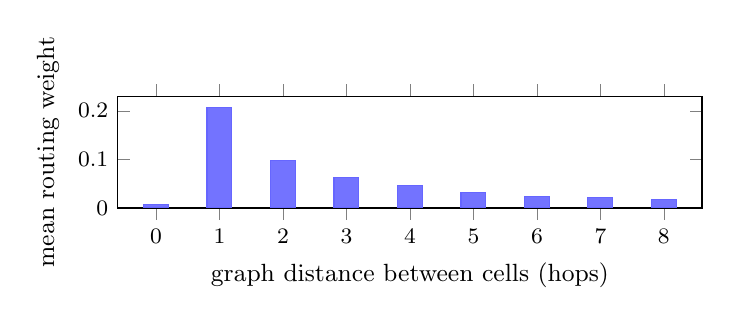
\begin{tikzpicture}
\begin{axis}[ybar,width=9cm,height=3.0cm,xlabel={graph distance between cells (hops)},ylabel={mean routing weight},
  xmin=-0.6,xmax=8.6,ymin=0,ymax=0.23,bar width=9pt,xtick={0,1,2,3,4,5,6,7,8},
  tick label style={font=\footnotesize},label style={font=\small}]
\addplot[fill=blue!55,draw=blue!60] coordinates {(0,0.007)(1,0.206)(2,0.098)(3,0.062)(4,0.047)(5,0.031)(6,0.024)(7,0.021)(8,0.018)};
\end{axis}\end{tikzpicture}
\caption{\textbf{The learned graph (recovery of $\mathcal{N}$).} Mean routing
(attention) weight vs graph distance between cells, on the \emph{dense} core:
geometric decay ($\rho\approx0.66$, reach $\sim$3 hops), ${\approx}0$ weight to
graph-unreachable cells (across walls), a small ${+}0.07$ anchor on the goal cell.
The dense routing \emph{learns} the transition adjacency $\mathcal{N}$ rather than
receiving it as a mask.}
\label{fig:kernel}
\end{figure}

\subsection{Amortized policy evaluation; the decision refines over ticks}
\label{sec:emp-planning}

We then ask what the thinking ticks actually compute (Prop.~\ref{prop:improvement}).
The precise finding, which we state carefully: the value field is computed in
essentially \emph{one} compiled step (amortized), and what the extra ticks refine
is the \emph{decision} --- most for the hardest states (Fig.~\ref{fig:refine}).

\textbf{(i) The operator has the form of a policy-evaluation backup, applied
amortized.} The routing operator is stationary across ticks
($\cos(\alpha^{k},\alpha^{k-1})\to0.995$; top-1 mass ${\approx}0.16$ over
${\sim}85$ keys; no sharpening), and the aggregation is a convex average (entmax,
\emph{not} $\max$): the \emph{form} of a soft policy-evaluation backup
$c\leftarrow\gamma_{\mathrm{eff}}\alpha c+r$, not value iteration. But it is
applied in essentially one step. Decoding the value field per tick and regressing
it on the model's \emph{own} operator applied to the previous tick,
$v_{t}\approx a\,(\alpha\,v_{t-1})+b\,v_{t-1}$, gives a propagation coefficient
$a$ that is nonzero \emph{only on the first tick} ($a{\approx}0.23\!\to\!0$), and
the per-cell value field is static thereafter
($\lVert\Delta v\rVert/\lVert v\rVert:0.01\!\to\!0$). So the value is
\emph{amortized} --- computed by the first tick, not iteratively propagated across
ticks (the same holds on a box-pushing value target, and on the convolutional
planner of \S\ref{sec:emp-drc}).

\textbf{(ii) The value field is a correct, causal value.} It is
Bellman-self-consistent (optimality residual$/\mathrm{std}(V)=[0.19,0.25,0.25,0.22]$
over greedy successors $0$--$3$) and consistent with one-step lookahead over its
own value. It is causal: moving the goal/box shifts $V$ in the resolvent-predicted
direction (a box edit more than a goal edit, $1.5\sigma$ vs $1.0\sigma$); a wall
that lengthens the agent's path lowers $V$ ($1.3\sigma$ vs $0.35\sigma$ off-path),
reaches the agent's \emph{own} cell ($2.2\times$) and re-plans its move ($3\times$
a cosmetic wall). The plan field $g^{k}$ (Def.~\ref{def:planfield}) is decodable
per cell as this value's gradient ($0.44$, chance $0.25$; $61\%$ goalward), and is
the attention pattern --- but it too is flat across ticks (no outward frontier).

\textbf{(iii) What the ticks refine is the decision.} Reading the model's
\emph{own} actor head at each tick, the chosen action \emph{changes on $35\%$ of
boards} from the first tick to the settled one and grows more goalward
($0.52\to0.60$, chance $0.25$); the decision margin sharpens ($1.6\to3.3$) and the
global value contracts ($|\Delta V|\,0.72\to0.23$), as the hidden settles toward a
fixed point ($\rho{\approx}0.89$). The gain is \emph{largest where the goal is
farthest} (${+}0.15$ at distance $\geq13$ vs ${+}0.07$--$0.10$ nearer). So the
extra test-time compute refines the \emph{decision} (and the hardest-state plan),
not the value field --- which is why thinking helps most on hard levels yet the
value field looks static. This is the improvement half of
Prop.~\ref{prop:improvement} realised at the head, over an amortized evaluation.

\begin{figure}[t]
\begin{subfigure}{0.32\textwidth}\centering
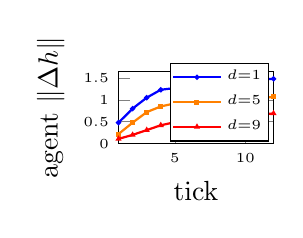
\begin{tikzpicture}
\begin{axis}[width=3.55cm,height=2.5cm,xlabel={tick},ylabel={agent $\lVert\Delta h\rVert$},
  xmin=1,xmax=12,ymin=0,ymax=1.65,legend pos=south east,legend style={font=\tiny,inner sep=0.6pt},
  tick label style={font=\tiny},label style={font=\tiny},xlabel near ticks,ylabel near ticks]
\addplot[mark=*,blue,thick,mark size=0.5pt] coordinates {(1,0.48)(2,0.80)(3,1.05)(4,1.23)(5,1.27)(6,1.31)(7,1.37)(8,1.42)(9,1.41)(10,1.44)(11,1.46)(12,1.48)};
\addplot[mark=square*,orange,thick,mark size=0.5pt] coordinates {(1,0.22)(2,0.48)(3,0.72)(4,0.85)(5,0.92)(6,0.97)(7,1.00)(8,0.99)(9,1.03)(10,1.03)(11,1.03)(12,1.07)};
\addplot[mark=triangle*,red,thick,mark size=0.5pt] coordinates {(1,0.11)(2,0.20)(3,0.31)(4,0.42)(5,0.49)(6,0.51)(7,0.53)(8,0.57)(9,0.58)(10,0.64)(11,0.66)(12,0.69)};
\legend{$d{=}1$,$d{=}5$,$d{=}9$}
\end{axis}\end{tikzpicture}
\vspace{-4pt}
\subcaption{a far perturbation's influence reaches the agent over several ticks (a transient).}
\label{fig:reach}
\end{subfigure}\hfill
\begin{subfigure}{0.32\textwidth}\centering
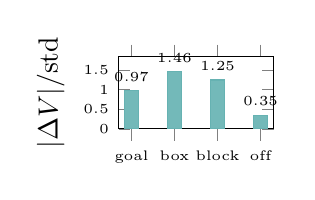
\begin{tikzpicture}
\begin{axis}[ybar,width=3.55cm,height=2.5cm,symbolic x coords={goal,box,block,off},xtick=data,
  ylabel={$|\Delta V|/\mathrm{std}$},ymin=0,ymax=1.85,bar width=5pt,
  nodes near coords,every node near coord/.append style={font=\tiny},
  tick label style={font=\tiny},label style={font=\tiny},ylabel near ticks]
\addplot[fill=teal!55,draw=teal!60] coordinates {(goal,0.97)(box,1.46)(block,1.25)(off,0.35)};
\end{axis}\end{tikzpicture}
\vspace{-4pt}
\subcaption{value tracks source/graph edits, not a cosmetic wall.}
\label{fig:abl}
\end{subfigure}\hfill
\begin{subfigure}{0.32\textwidth}\centering
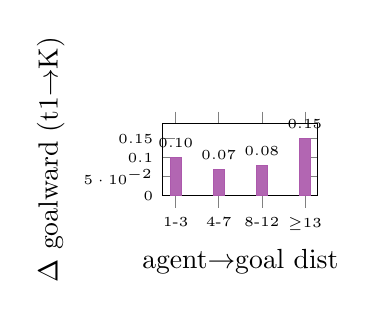
\begin{tikzpicture}
\begin{axis}[ybar,width=3.55cm,height=2.5cm,symbolic x coords={1-3,4-7,8-12,$\geq$13},xtick=data,
  ylabel={$\Delta$ goalward (t1$\to$K)},ymin=0,ymax=0.19,bar width=4pt,xlabel={agent$\to$goal dist},
  nodes near coords,every node near coord/.append style={font=\tiny,/pgf/number format/.cd,fixed,fixed zerofill,precision=2},
  tick label style={font=\tiny},label style={font=\tiny},xlabel near ticks,ylabel near ticks]
\addplot[fill=violet!60,draw=violet!65] coordinates {(1-3,0.10)(4-7,0.07)(8-12,0.08)($\geq$13,0.15)};
\end{axis}\end{tikzpicture}
\vspace{-4pt}
\subcaption{the decision turns goalward over ticks, most when the goal is far.}
\label{fig:decide}
\end{subfigure}
\caption{\textbf{Amortized value; the decision refines over ticks.} (a) a far
perturbation's influence reaches the agent over a few ticks (a transient --- the value
field itself is amortized, set by tick~1); (b) the value causally tracks edits to the
source (goal/box) and the graph (a path-blocking wall) --- reaching the agent and
re-planning --- but not a cosmetic off-path wall; (c) reading the model's own head per
tick, the \emph{decision} becomes more goalward as the hidden settles, the gain largest
where the goal is farthest.}
\label{fig:refine}
\end{figure}

\textbf{The spatial form of the improvement is routing-dependent.}
Prop.~\ref{prop:improvement} pictures $g^{k}$ \emph{expanding by one transition
per thinking step} --- a ring-by-ring wavefront. That is the signature of
\emph{local} routing: a masked/convolutional core relays one hop per step, and is
exactly what prior work decodes from convolutional planners, where directional,
square-attached plan concepts grow outward over internal ticks
\citep{bush2025interpreting,taufeeque2024planning}. In the \emph{dense} core,
routing is global at every step, so a single step already backs the field up over
all feasible neighbours board-wide; we accordingly find \emph{no} staggered
near$\to$far frontier --- the per-cell plan field is established early and is flat
across thinking steps (replicated at $192$ and $512$ boards). The improvement is
realised globally instead, as the distance-scaled \emph{decision} change of part
(iii). The dense core thus realises the depth-$K$ improvement of
Prop.~\ref{prop:improvement} \emph{without} a spatial wavefront: the wavefront is
specific to local routing, the improvement content is not.

\paragraph{Summary.} In the fully-learned instance, an attention core given only
RL signal discovers a binding $\sigma$ (\S\ref{sec:emp-binding}) and a routing
that recovers $\mathcal{N}$ (\S\ref{sec:emp-routing}), and runs an \emph{amortized}
policy-evaluation operator whose \emph{decision} it then refines over thinking
ticks (\S\ref{sec:emp-planning}) --- generalized policy iteration with the
evaluation compiled into the forward pass and the improvement at the head. It
exhibits the same planning content prior work decodes from convolutional planners
\citep{guez2019investigation,bush2025interpreting,taufeeque2024planning}, but with
the binding and the propagation both \emph{learned} rather than handed to the
network by spatial weight-sharing and a local stencil --- the generalization this
paper claims. Table~\ref{tab:empirics} collects the measurements; full per-probe
detail is in App.~\ref{app:experiments}.

\begin{table}[t]
\centering\small
\caption{Mechanistic measurements on the trained dense attention core (held-out
Sokoban, $300\mathrm{M}$-step checkpoint). Each row is a probe in
\texttt{experiments/interp/}; ``chance'' is the trivial baseline.}
\label{tab:empirics}
\resizebox{\linewidth}{!}{%
\begin{tabular}{@{}lll@{}}
\toprule
Prediction & Measurement & Result \\
\midrule
Binding (Def.~\ref{def:indexed}) & decode state from one cell $h_t(\sigma(s))$ & $0.74/0.73/0.72/0.78$ (chance $0.50$), flat in $k$ \\
Recovery of $\mathcal{N}$ & routing mass on feasible neighbours & $7$--$13\times$ uniform; $\rho{\approx}0.66$; ${\approx}0$ thru walls \\
\quad (causal) & wall-blocked vs.\ graph-near influence & $0.38\times$; partial corr.\ $-0.32$ \\
Operator (PE-backup form) & stationarity; aggregation & $\cos\to0.995$; convex average (no $\max$) \\
Value amortized & $\lVert\Delta v\rVert$/tick; own-operator coeff $a$ & $0.01{\to}0$; $a{=}0.23$ tick~1 ${\to}\,0$ \\
Bellman consistency & optimality residual$/\mathrm{std}(V)$ & $[0.19,0.25,0.25,0.22]$ over successors $0$--$3$ \\
Causal value$\to$action & path-block wall: $\Delta V$; re-plan rate & $-1.3\sigma$ vs.\ $-0.35\sigma$; $2.2\times$/$3\times$ \\
Plan field $=$ routing & per-cell action $=$ value gradient & $0.44$ (chance $0.25$); $61\%$ goalward, flat in $k$ \\
Decision refines over ticks & action change; margin; goalward by dist. & $35\%$ change; margin $1.6{\to}3.3$; $+0.15$ at dist.\ $\geq13$ \\
\bottomrule
\end{tabular}}
\end{table}


\subsection{Cross-check: cellwise GPI in the convolutional planner}
\label{sec:emp-drc}

If relational latent states are the operative bias, the \emph{masked} (convolutional) instance studied by
prior work should show the same cellwise GPI --- now with the routing graph $\mathcal{N}$ supplied by the
conv stencil rather than learned. We test this directly on the pretrained DRC(3,3) of
\citet{guez2019investigation} (the $2\mathrm{B}$-step checkpoint interpreted by
\citet{bush2025interpreting,taufeeque2024planning}), probing its per-cell ConvLSTM hidden over thinking ticks
against the \emph{box-pushing} ground truth (per cell: box-push distance to the nearest target, and the
optimal first-push direction).

\textbf{The cellwise fixed point is present.} Each cell carries a decodable value statistic whose
\emph{gradient is the optimal push direction $75\%$ of the time}, and a decodable greedy push-direction
(accuracy $0.68$, chance $0.25$) that agrees with that value gradient ($0.55$): a per-cell value together
with a policy greedy with respect to it --- exactly the policy-iteration fixed point of
Section~\ref{sec:planning}, here laid out explicitly at each board square (the directional, square-attached
``plan'' concepts of \citet{bush2025interpreting}). \textbf{It is causal:} a wall that lengthens the box-push
path re-forms the decoded cellwise value $2.5$--$5\times$ more than a cosmetic wall, in the direction the new
physics predicts.

\textbf{Amortized, with distance-graded refinement.} At $2\mathrm{B}$ steps the per-cell value is
\emph{amortized} --- the same direct test as \S\ref{sec:emp-planning}(i) finds the decoded value propagated by
the core's own (local) operator only on the first tick and static thereafter ($\lVert\Delta v\rVert\!\to\!0$).
Additional thinking refines mainly the \emph{far} cells (push-distance $6$--$8$: direction accuracy
$0.46\!\to\!0.69$ over ticks) and the causal response is front-loaded. This mirrors the dense core
(\S\ref{sec:emp-planning}): both compute the value field in essentially one compiled step, with thinking
buying the largest decision/plan gain for the far / hard states.

\textbf{One mechanism, two routing regimes.} Masked and dense instances both carry a cellwise value and a
cellwise greedy policy that is its gradient --- GPI on the learned graph. What the routing regime sets is the
\emph{form}: with local (conv) routing the per-cell plan is explicit and refines as a (weak) outward frontier
\citep{bush2025interpreting,taufeeque2024planning}; with dense routing the per-cell plan is weaker and the
improvement also surfaces at the head (\S\ref{sec:emp-planning}), with no spatial frontier. The shared
invariant is GPI; locality decides only how it is spatially realised. (The box-push distance is an optimistic
proxy that ignores agent reachability, and the value $R^2$ is modest --- the direction accuracy $0.68$ and
value-gradient${=}$optimal $0.75$ are the load-bearing numbers.)

\section{Discussion \& Future Work}
\label{sec:discussion}

\begin{ack}
The author is supported by an Excellence Scholarship of the State of Lower Austria.
\end{ack}

\bibliographystyle{plainnat}
\bibliography{references}

\newpage
\appendix
\onecolumn

\section{Architecture and training of the attention instance}
\label{app:arch}

The core is the dense (attention) instance of Assumption~\ref{ass:core}. The
$N=100$ latent cells are the squares of the $10\times10$ board; the recurrent
carry is, per stacked cell $d\in\{0,1,2\}$ ($D=3$), a memory $c_d$ and hidden
$h_d$ in $\mathbb{R}^{N\times C}$ ($C=32$), with $x\in\mathbb{R}^{N\times C}$ a
convolutional board embedding fixed across thinking steps. Each thinking step
applies, for $d=0,1,2$ bottom-to-top (with $\mathrm{prev}$ the hidden of the cell
below, or the previous step's top hidden for $d{=}0$), the weight-tied update
\begin{align*}
  u &= \mathrm{RMSNorm}\!\bigl(h_d + [x;\mathrm{prev}]W_{\mathrm{in}}^{d} + b^{d}\bigr)\odot s^{d},\\
  q,k,v &= uW_q^{d},\; uW_k^{d},\; uW_v^{d}\quad(\text{$4$ heads, }d_h{=}8),\\
  \alpha &= \mathrm{entmax}_{1.5}\!\bigl(qk^{\top}/\sqrt{d_h}+\mathrm{RelBias}^{d}\bigr),\qquad
  z=(\alpha\,v)\,W_{\mathrm{out}}^{d},\\
  [g_i,g_j,g_f,g_o] &= [x;\mathrm{prev};z]\,W_g^{d}+b_g^{d},\\
  c_d &\leftarrow c_d\,\sigma(g_f)+\tanh(g_i)\,\sigma(g_j),\qquad
  h_d \leftarrow \tanh(c_d)\odot\tanh(g_o).
\end{align*}
Here $\alpha$ is the content-based routing of \eqref{eq:update} (row-stochastic;
dense over all $N$ cells; sparse via the $1.5$-entmax normaliser, which sends most
weights to exactly zero) and $z$ is the convex-average aggregation $\oplus$ (no
$\max$). The loop runs up to $K=6$ steps. The per-board readout pools cells into
$m=\mathrm{ReLU}\bigl((h_2+x)W_{\mathrm{dense}}+b\bigr)$, then actor logits
$mW_a+b_a$ and critic value $V=(mW_c+b_c)\,s_{\mathrm{head}}$ --- the localized
readouts $\rho_\pi,\rho_V$ of Def.~\ref{def:localized}. Training is IMPALA on
Boxoban unfiltered-train, $300\mathrm{M}$ steps, $\gamma=0.97$, thinking depth
$\sim\mathcal U\{1..6\}$ per rollout (the learner replays the same depth); online
train solve $\approx83\%$, held-out medium solve $\approx31\%$. All probes use the
held-out medium split at the $300\mathrm{M}$ checkpoint.

\section{Faithful recompute}
\label{app:recompute}

The model's own forward hits a tracer error on the offset-tied $\mathrm{RelBias}$
gather under its scan, so every probe recomputes the $D{=}3$ entmax stack above in
plain JAX from the loaded parameters and verifies that the recomputed final hidden
state matches the model's to $1.8\times10^{-7}$. The extracted routing and cell
states are therefore the model's, not a re-implementation artifact.

\section{Experiment catalog}
\label{app:experiments}

Scripts are under \texttt{experiments/interp/} and run as
\texttt{python -m experiments.interp.<name>}; weights are under
\texttt{checkpoints/}. Each loads the $300\mathrm{M}$ checkpoint, recomputes the
core (App.~\ref{app:recompute}), and prints its measurement.

\textbf{Binding (\S\ref{sec:emp-binding}).}
\texttt{planning.py} --- linear probe $h_t(\sigma(s))\!\to\!$ state content,
per-object balanced accuracy, per thinking step.

\textbf{Recovery of $\mathcal{N}$ (\S\ref{sec:emp-routing}).}
\texttt{planning.py} (routing mass on feasible move-neighbours vs.\ uniform);
\texttt{e4.py} (routing weight vs.\ graph distance: $\rho{\approx}0.66$, ${\approx}0$
beyond the graph, ${+}0.07$ to the goal); \texttt{wall.py} (through-walls,
causal: blocked vs.\ open influence at matched pixel distance);
\texttt{perturb.py}, \texttt{topo.py} (causal influence radius vs.\ steps; graph-
vs.\ Euclidean-distance).

\textbf{Propagated improvement (\S\ref{sec:emp-planning}).}
\texttt{e1.py} (operator stationarity; convex average $\Rightarrow$ evaluation, not
in-loop value iteration); \texttt{e5.py} (reach compounds with steps);
\texttt{bellman.py} (optimality residual at agent and greedy successors);
\texttt{lookahead.py} (policy vs.\ one-step lookahead over the model's own value,
by depth); \texttt{e2.py} (reward-relabel: policy-evaluation vs.\ successor
representation); \texttt{e6.py}, \texttt{e6b.py} (goal/box edits shift $V$ in the
resolvent-predicted direction; box $>$ goal); \texttt{e7.py}, \texttt{e7b.py} (the
routing does \emph{not} re-wire under a single edit --- propagation is by content,
not re-routing); \texttt{e8.py} (value-projection norm by tile; wall cells are not
``dead''); \texttt{e9.py} (a path-blocking wall lowers $V$, building over steps);
\texttt{e10.py} (the wall's value-change reaches the agent's cell and re-plans its
move); \texttt{e11.py} (the plan field $g^{k}$ is decodable per cell as the value
gradient --- for attention, it is the routing pattern); \texttt{e12.py} (the
per-cell field does \emph{not} expand as a spatial frontier over steps --- the
expected signature of a \emph{dense} core, which propagates globally per step);
\texttt{e13.py} (the agent's own decision changes and improves over steps, most on
the farthest states; value contracts and the margin sharpens). \texttt{e3.py} is a
no-kinks behavioural check; \texttt{planq.py} confirms only the immediate action
(not a stored multi-step action sequence) is decodable.

\end{document}
